\let\negmedspace\undefined
\let\negthickspace\undefined
\documentclass[journal]{IEEEtran}
\usepackage[a5paper, margin=10mm, onecolumn]{geometry}
%\usepackage{lmodern} % Ensure lmodern is loaded for pdflatex
\usepackage{tfrupee} % Include tfrupee package

\setlength{\headheight}{1cm} % Set the height of the header box
\setlength{\headsep}{0mm}     % Set the distance between the header box and the top of the text

\usepackage{gvv-book}
\usepackage{gvv}
\usepackage{cite}
\usepackage{amsmath,amssymb,amsfonts,amsthm}
\usepackage{algorithmic}
\usepackage{graphicx}
\usepackage{textcomp}
\usepackage{xcolor}
\usepackage{txfonts}
\usepackage{listings}
\usepackage{enumitem}
\usepackage{mathtools}
\usepackage{gensymb}
\usepackage{comment}
\usepackage[breaklinks=true]{hyperref}
\usepackage{tkz-euclide} 
\usepackage{listings}
% \usepackage{gvv}                                        
\def\inputGnumericTable{}                                 
\usepackage[latin1]{inputenc}                                
\usepackage{color}                                            
\usepackage{array}                                            
\usepackage{longtable}                                       
\usepackage{calc}                                             
\usepackage{multirow}                                         
\usepackage{hhline}                                           
\usepackage{ifthen}                                           
\usepackage{lscape}
\begin{document}

\bibliographystyle{IEEEtran}
\vspace{3cm}

\title{1-1.2-28}
\author{EE24BTECH11036 - Krishna Patil}
% \maketitle
% \newpage
% \bigskip
{\let\newpage\relax\maketitle}

\renewcommand{\thefigure}{\theenumi}
\renewcommand{\thetable}{\theenumi}
\setlength{\intextsep}{10pt} % Space between text and floats


\numberwithin{equation}{enumi}
\numberwithin{figure}{enumi}
\renewcommand{\thetable}{\theenumi}
\parindent 0px 
{Question :-} \\ 
 In which quadrant or on which axis do each of the points {$ \brak{-2,4 }$}, {$ \brak{3,-1} $}, {$ \brak{-1,0} $}, {$ \brak{1,2} $} and {$ \brak{-3,-5} $} lie ? Verify your answer by locating them on the Cartesian plane. \\ \\
\solution \\
To determine if point lies in a quadrant , we look at the the signs of the x and y coordinates as shown in the table \ref{tab1-1.2-28}. \\
\begin{table}[h!]    
  \centering
  \begin{tabular}[12pt]{ |c| c| c|} 
    \hline
    {Sign of X coordinate} & {Sign of Y coordinate} & {Quadrant or Axis}\\ 
    \hline
    $ + $ & $ + $ & $ Q_1 $\\
    \hline 
    $ - $ & $ + $ & $ Q_2 $ \\
    \hline
    $ - $ & $ - $ & $ Q_3 $ \\
    \hline   
    $ + $ & $ - $ & $ Q_4 $\\
    \hline
    any  & $ 0 $ & x-axis\\
    \hline
    $ 0 $ &  any  & y-axis\\
    \hline
    \end{tabular}

  \caption{Quadrant Decider}
  \label{tab1-1.2-28}
\end{table} \\
\begin{figure}[h!]
   \parindent 1px
	\centering
	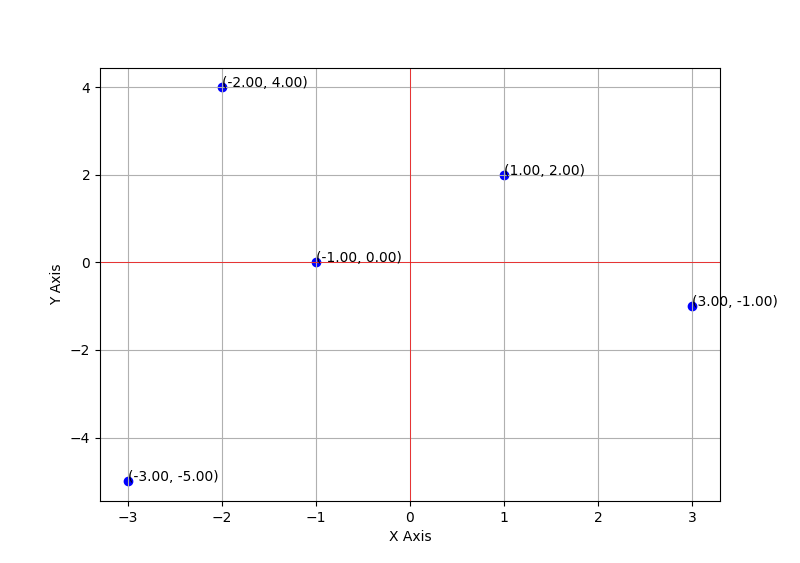
\includegraphics[width=0.5\linewidth]{figs/Figure_1.png}
   \caption{X-Y plot}
   \label{x-yplot}
\end{figure} \\ \\ 
\newpage
So , By \ref{x-yplot} ,the table \ref{Answers} gives the answers.
\begin{table}[h!]    
  \centering
  \begin{tabular}[12pt]{ |c| c| c|} 
    \hline
    {Point} & {Value} & {Quadrant or Axis}\\ 
    \hline
    $ \vec{A} $ & $ \brak{-2,4} $ & $ Q_2 $ \\
    \hline 
    $ \vec{B} $ & $ \brak{3,-1} $ & $ Q_4 $ \\
    \hline
    $ \vec{C} $ & $ \brak{-1,0} $ & x-axis \\
    \hline   
    $ \vec{D} $ & $ \brak{1,2} $ & $ Q_1 $ \\
    \hline
    $ \vec{E} $ & $ \brak{-3,-5} $ &   $ Q_3 $ \\
    \hline
    \end{tabular}
  \caption{Answers}
  \label{Answers}
\end{table}
\end{document}
